\documentclass[border=10pt]{standalone}
\usepackage{tikz}
\usetikzlibrary{shapes.geometric, arrows.meta, positioning, calc, fit, backgrounds}

% Define styles
\tikzset{
    block/.style={
        rectangle,
        draw=black,
        thick,
        fill=white,
        minimum width=1.8cm,
        minimum height=1cm,
        align=center,
        font=\small\bfseries
    },
    smallblock/.style={
        rectangle,
        draw=black,
        thick,
        fill=gray!20,
        minimum width=1cm,
        minimum height=0.7cm,
        align=center,
        font=\scriptsize\bfseries
    },
    pool/.style={
        rectangle,
        draw=black,
        thick,
        fill=gray!40,
        minimum width=0.8cm,
        minimum height=0.6cm,
        align=center,
        font=\scriptsize
    },
    attention/.style={
        rectangle,
        draw=black,
        thick,
        fill=black!80,
        text=white,
        minimum width=0.9cm,
        minimum height=0.5cm,
        align=center,
        font=\scriptsize\bfseries
    },
    arrow/.style={
        ->,
        >=Stealth,
        thick
    },
    skiparrow/.style={
        ->,
        >=Stealth,
        thick,
        dashed
    },
    label/.style={
        font=\scriptsize,
        text=gray
    }
}

\begin{document}

%% ============================================================================
%% V1: BASELINE CNN
%% ============================================================================
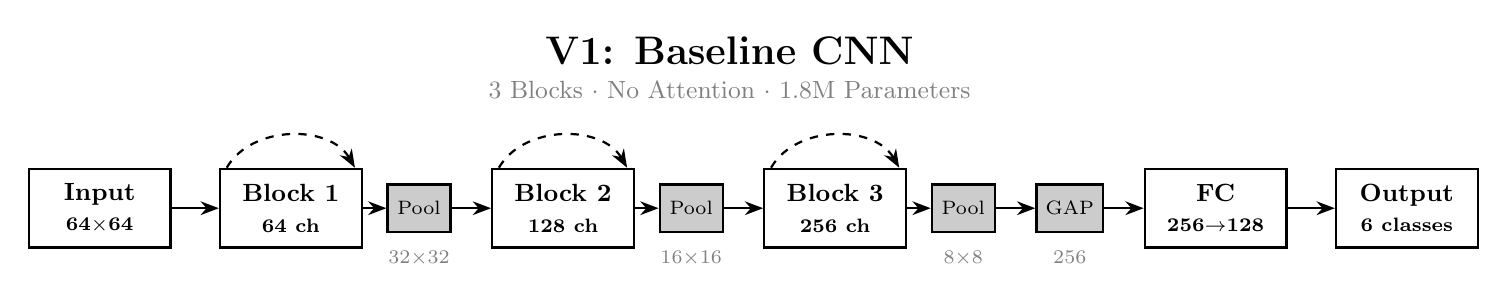
\begin{tikzpicture}[node distance=0.6cm]

    % Title
    \node[font=\Large\bfseries] at (8, 2) {V1: Baseline CNN};
    \node[font=\small, text=gray] at (8, 1.5) {3 Blocks $\cdot$ No Attention $\cdot$ 1.8M Parameters};

    % Input
    \node[block] (input) at (0, 0) {Input\\{\scriptsize 64$\times$64}};

    % Block 1
    \node[block, right=of input] (b1) {Block 1\\{\scriptsize 64 ch}};
    \node[pool, right=0.3cm of b1] (p1) {Pool};
    \node[label, below=0.1cm of p1] {32$\times$32};

    % Block 2
    \node[block, right=0.5cm of p1] (b2) {Block 2\\{\scriptsize 128 ch}};
    \node[pool, right=0.3cm of b2] (p2) {Pool};
    \node[label, below=0.1cm of p2] {16$\times$16};

    % Block 3
    \node[block, right=0.5cm of p2] (b3) {Block 3\\{\scriptsize 256 ch}};
    \node[pool, right=0.3cm of b3] (p3) {Pool};
    \node[label, below=0.1cm of p3] {8$\times$8};

    % GAP
    \node[pool, right=0.5cm of p3] (gap) {GAP};
    \node[label, below=0.1cm of gap] {256};

    % FC
    \node[block, right=0.5cm of gap] (fc) {FC\\{\scriptsize 256$\to$128}};

    % Output
    \node[block, right=of fc] (output) {Output\\{\scriptsize 6 classes}};

    % Arrows
    \draw[arrow] (input) -- (b1);
    \draw[arrow] (b1) -- (p1);
    \draw[arrow] (p1) -- (b2);
    \draw[arrow] (b2) -- (p2);
    \draw[arrow] (p2) -- (b3);
    \draw[arrow] (b3) -- (p3);
    \draw[arrow] (p3) -- (gap);
    \draw[arrow] (gap) -- (fc);
    \draw[arrow] (fc) -- (output);

    % Skip connections
    \draw[skiparrow] ($(b1.north west)+(0.1,0)$) to[out=60,in=120] ($(b1.north east)+(-0.1,0)$);
    \draw[skiparrow] ($(b2.north west)+(0.1,0)$) to[out=60,in=120] ($(b2.north east)+(-0.1,0)$);
    \draw[skiparrow] ($(b3.north west)+(0.1,0)$) to[out=60,in=120] ($(b3.north east)+(-0.1,0)$);

\end{tikzpicture}

\newpage

%% ============================================================================
%% V2: SE ATTENTION
%% ============================================================================
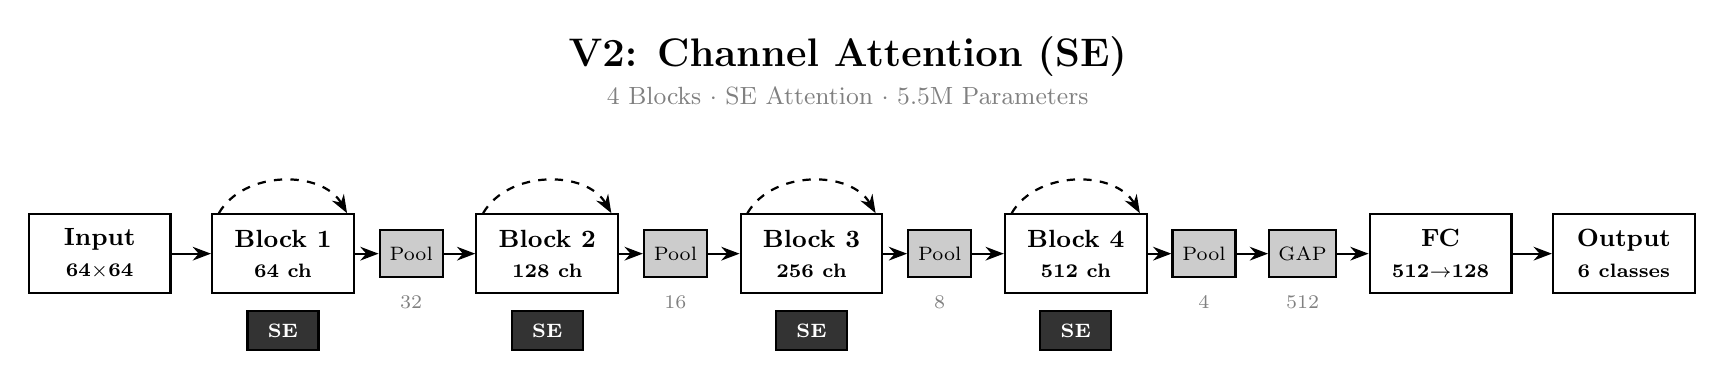
\begin{tikzpicture}[node distance=0.5cm]

    % Title
    \node[font=\Large\bfseries] at (9.5, 2.5) {V2: Channel Attention (SE)};
    \node[font=\small, text=gray] at (9.5, 2) {4 Blocks $\cdot$ SE Attention $\cdot$ 5.5M Parameters};

    % Input
    \node[block] (input) at (0, 0) {Input\\{\scriptsize 64$\times$64}};

    % Block 1 + SE
    \node[block, right=of input] (b1) {Block 1\\{\scriptsize 64 ch}};
    \node[attention, below=0.2cm of b1] (se1) {SE};
    \node[pool, right=0.3cm of b1] (p1) {Pool};
    \node[label, below=0.1cm of p1] {\scriptsize 32};

    % Block 2 + SE
    \node[block, right=0.4cm of p1] (b2) {Block 2\\{\scriptsize 128 ch}};
    \node[attention, below=0.2cm of b2] (se2) {SE};
    \node[pool, right=0.3cm of b2] (p2) {Pool};
    \node[label, below=0.1cm of p2] {\scriptsize 16};

    % Block 3 + SE
    \node[block, right=0.4cm of p2] (b3) {Block 3\\{\scriptsize 256 ch}};
    \node[attention, below=0.2cm of b3] (se3) {SE};
    \node[pool, right=0.3cm of b3] (p3) {Pool};
    \node[label, below=0.1cm of p3] {\scriptsize 8};

    % Block 4 + SE
    \node[block, right=0.4cm of p3] (b4) {Block 4\\{\scriptsize 512 ch}};
    \node[attention, below=0.2cm of b4] (se4) {SE};
    \node[pool, right=0.3cm of b4] (p4) {Pool};
    \node[label, below=0.1cm of p4] {\scriptsize 4};

    % GAP
    \node[pool, right=0.4cm of p4] (gap) {GAP};
    \node[label, below=0.1cm of gap] {512};

    % FC
    \node[block, right=0.4cm of gap] (fc) {FC\\{\scriptsize 512$\to$128}};

    % Output
    \node[block, right=of fc] (output) {Output\\{\scriptsize 6 classes}};

    % Main arrows
    \draw[arrow] (input) -- (b1);
    \draw[arrow] (b1) -- (p1);
    \draw[arrow] (p1) -- (b2);
    \draw[arrow] (b2) -- (p2);
    \draw[arrow] (p2) -- (b3);
    \draw[arrow] (b3) -- (p3);
    \draw[arrow] (p3) -- (b4);
    \draw[arrow] (b4) -- (p4);
    \draw[arrow] (p4) -- (gap);
    \draw[arrow] (gap) -- (fc);
    \draw[arrow] (fc) -- (output);

    % Skip connections
    \draw[skiparrow] ($(b1.north west)+(0.1,0)$) to[out=60,in=120] ($(b1.north east)+(-0.1,0)$);
    \draw[skiparrow] ($(b2.north west)+(0.1,0)$) to[out=60,in=120] ($(b2.north east)+(-0.1,0)$);
    \draw[skiparrow] ($(b3.north west)+(0.1,0)$) to[out=60,in=120] ($(b3.north east)+(-0.1,0)$);
    \draw[skiparrow] ($(b4.north west)+(0.1,0)$) to[out=60,in=120] ($(b4.north east)+(-0.1,0)$);

\end{tikzpicture}

\newpage

%% ============================================================================
%% V3: DUAL ATTENTION
%% ============================================================================
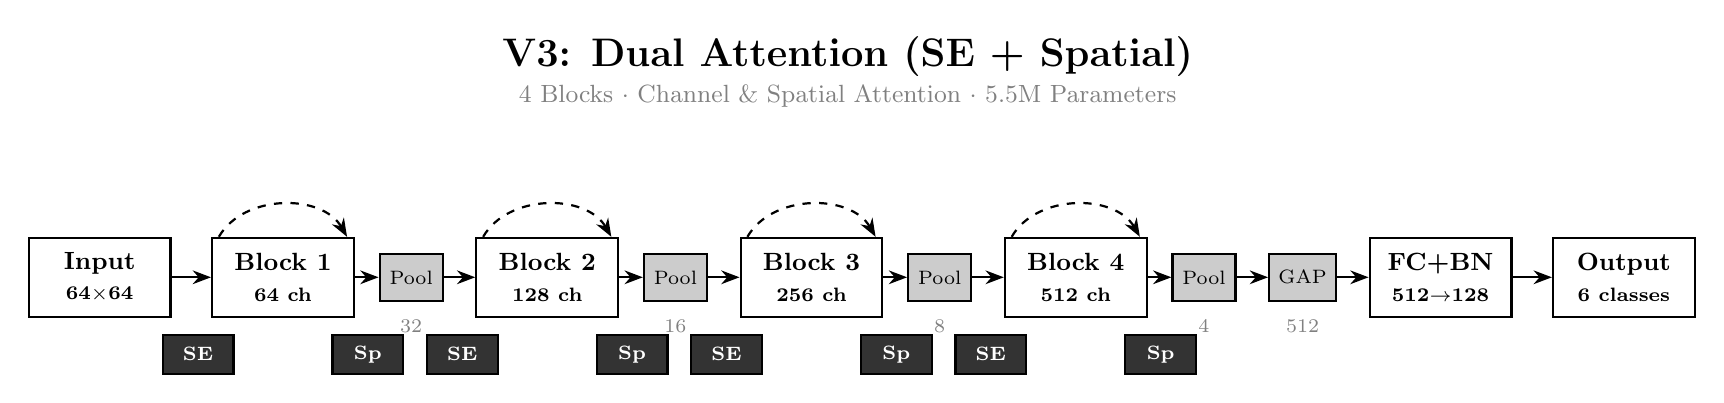
\begin{tikzpicture}[node distance=0.5cm]

    % Title
    \node[font=\Large\bfseries] at (9.5, 2.8) {V3: Dual Attention (SE + Spatial)};
    \node[font=\small, text=gray] at (9.5, 2.3) {4 Blocks $\cdot$ Channel \& Spatial Attention $\cdot$ 5.5M Parameters};

    % Input
    \node[block] (input) at (0, 0) {Input\\{\scriptsize 64$\times$64}};

    % Block 1 + Dual Attention
    \node[block, right=of input] (b1) {Block 1\\{\scriptsize 64 ch}};
    \node[attention, below left=0.2cm and -0.3cm of b1] (se1) {SE};
    \node[attention, below right=0.2cm and -0.3cm of b1] (sp1) {Sp};
    \node[pool, right=0.3cm of b1] (p1) {Pool};
    \node[label, below=0.1cm of p1] {\scriptsize 32};

    % Block 2 + Dual Attention
    \node[block, right=0.4cm of p1] (b2) {Block 2\\{\scriptsize 128 ch}};
    \node[attention, below left=0.2cm and -0.3cm of b2] (se2) {SE};
    \node[attention, below right=0.2cm and -0.3cm of b2] (sp2) {Sp};
    \node[pool, right=0.3cm of b2] (p2) {Pool};
    \node[label, below=0.1cm of p2] {\scriptsize 16};

    % Block 3 + Dual Attention
    \node[block, right=0.4cm of p2] (b3) {Block 3\\{\scriptsize 256 ch}};
    \node[attention, below left=0.2cm and -0.3cm of b3] (se3) {SE};
    \node[attention, below right=0.2cm and -0.3cm of b3] (sp3) {Sp};
    \node[pool, right=0.3cm of b3] (p3) {Pool};
    \node[label, below=0.1cm of p3] {\scriptsize 8};

    % Block 4 + Dual Attention
    \node[block, right=0.4cm of p3] (b4) {Block 4\\{\scriptsize 512 ch}};
    \node[attention, below left=0.2cm and -0.3cm of b4] (se4) {SE};
    \node[attention, below right=0.2cm and -0.3cm of b4] (sp4) {Sp};
    \node[pool, right=0.3cm of b4] (p4) {Pool};
    \node[label, below=0.1cm of p4] {\scriptsize 4};

    % GAP
    \node[pool, right=0.4cm of p4] (gap) {GAP};
    \node[label, below=0.1cm of gap] {512};

    % FC
    \node[block, right=0.4cm of gap] (fc) {FC+BN\\{\scriptsize 512$\to$128}};

    % Output
    \node[block, right=of fc] (output) {Output\\{\scriptsize 6 classes}};

    % Main arrows
    \draw[arrow] (input) -- (b1);
    \draw[arrow] (b1) -- (p1);
    \draw[arrow] (p1) -- (b2);
    \draw[arrow] (b2) -- (p2);
    \draw[arrow] (p2) -- (b3);
    \draw[arrow] (b3) -- (p3);
    \draw[arrow] (p3) -- (b4);
    \draw[arrow] (b4) -- (p4);
    \draw[arrow] (p4) -- (gap);
    \draw[arrow] (gap) -- (fc);
    \draw[arrow] (fc) -- (output);

    % Skip connections
    \draw[skiparrow] ($(b1.north west)+(0.1,0)$) to[out=60,in=120] ($(b1.north east)+(-0.1,0)$);
    \draw[skiparrow] ($(b2.north west)+(0.1,0)$) to[out=60,in=120] ($(b2.north east)+(-0.1,0)$);
    \draw[skiparrow] ($(b3.north west)+(0.1,0)$) to[out=60,in=120] ($(b3.north east)+(-0.1,0)$);
    \draw[skiparrow] ($(b4.north west)+(0.1,0)$) to[out=60,in=120] ($(b4.north east)+(-0.1,0)$);

\end{tikzpicture}

\end{document}
